%%%%%%%%%%%%%%%%%%%%%%%%%%%%%%%%%%%%%%%%
\begin{figure*}[thb]
\centering
% 
\begin{subfigure}[b]{0.45\linewidth}
\centering
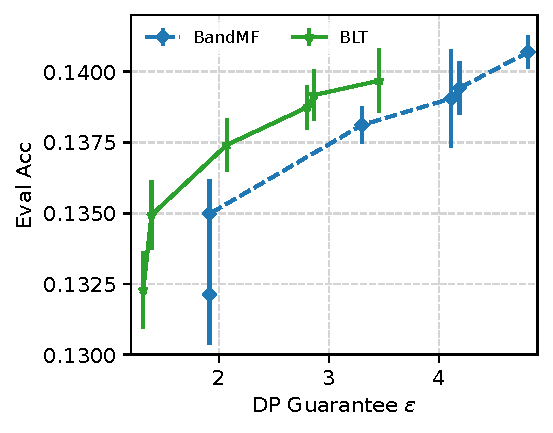
\includegraphics[width=\textwidth]{images/eses_priv.pdf}
\caption{\small Spanish LM in Spain (es-ES)}
\label{fig:es_priv}
\end{subfigure}
%
\begin{subfigure}[b]{0.45\linewidth}
\centering
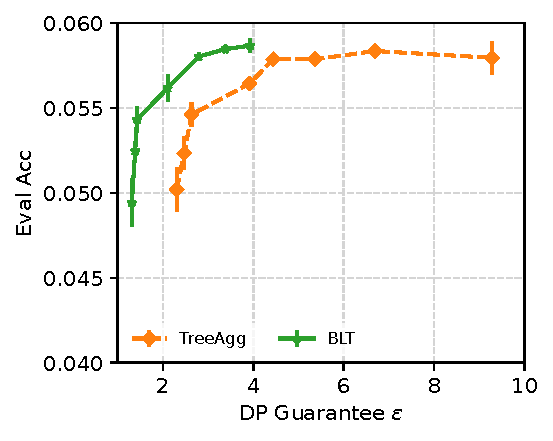
\includegraphics[width=\textwidth]{images/idid_priv.pdf}
\caption{\small Indonesian LM in Indonesia (id-ID)}
\label{fig:id_priv}
\end{subfigure}
%
\begin{subfigure}[b]{0.45\linewidth}
\centering
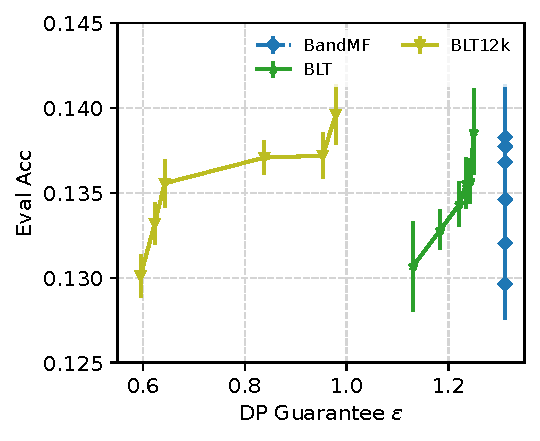
\includegraphics[width=\textwidth]{images/ptbr_priv.pdf}
\caption{\small Portuguese LM in Brazil (pt-BR)}
\label{fig:br_priv}
\end{subfigure}
%
\begin{subfigure}[b]{0.45\linewidth}
\centering
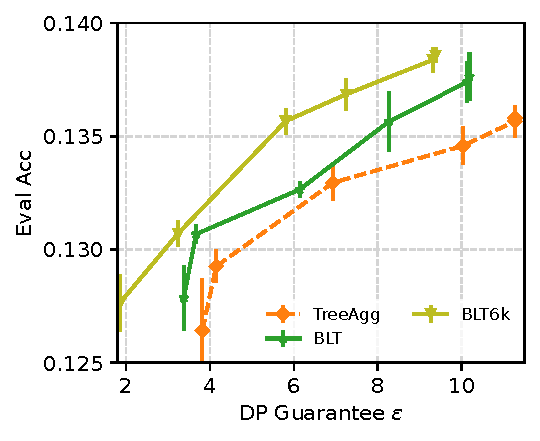
\includegraphics[width=\textwidth]{images/ptpt_priv.pdf}
\caption{\small Portuguese LM in Portugal (pt-PT)}
\label{fig:pt_priv}
\end{subfigure}
%
\caption{\small The privacy-utility trade-off curves derived from \cref{fig:acc_curve}. For each selected round $r$, we compute the mean and standard deviation (shown as vertical bars) for accuracy from the rounds in the range of $r\pm50$ ($r\pm10$ for pt-PT), and also accounting the DP guarantees. \blts show better privacy-utility trade-off as their curves are closer to the top left (small DP guarantees and large NWP accuracy).
}\label{fig:priv_curve}
\end{figure*}
%%%%%%%%%%%%%%%%%%%%%%%%%%%%%%